\documentclass[12pt,compress,aspectratio=169]{beamer}

\mode<presentation>
{
  \usetheme{Singapore}
%  \setbeamertemplate{navigation symbols}{} % suppress nav bar
%  \setbeamercovered{transparent}
}
\usefonttheme{professionalfonts}
\usepackage{graphicx}
\usepackage{tikz}
\usepackage{amsmath}
\usepackage{mathpazo}
\usepackage[scaled]{helvet}
\usepackage{xcolor,colortbl}
\usepackage{hyperref}
\usepackage{siunitx}

\sisetup{
  number-math-rm=\mathnormal,
  per-mode=symbol
}

\title{Topic 23: Special Relativity}
\subtitle{Advanced Placement Physics}
\author[TML]{Dr.\ Timothy Leung}
\institute{Olympiads School}
%\author{Olympiads School}
\date{Summer 2018}



\newcommand{\mb}[1]{\mathbf{#1}}
\newcommand{\pic}[2]{\includegraphics[width=#1\textwidth]{#2}}
\newcommand{\bigsqrt}{\ensuremath\sqrt{1-\left(\frac{v}{c}\right)^2}}
\newcommand{\lorentz}{\ensuremath\frac{1}{\bigsqrt}}
\newcommand{\eq}[2]{\vspace{#1}{\Large\begin{displaymath}#2\end{displaymath}}}



\begin{document}

\begin{frame}
  \maketitle
\end{frame}



\section[Intro]{Introduction}
\begin{frame}
  \frametitle{Introduction}
  These slides for this unit are an expanded version of Grade 12 Physics slides
  (with some additional calculus). Two versions of the slides are downloadable
  from the school website:
  \begin{itemize}
  \item The long version
    \begin{itemize}
    \item More background information (more than needed for the AP 2 Exam) and
      derivations and integrations
    \item May answer some of your questions about the specifics of the theory
    \item \texttt{23a-relativity\_long.pdf}
    \end{itemize}
  \item<alert@1> The short version
    \begin{itemize}
    \item More ``to the point''
    \item The version that is used during class
    \item \texttt{23a-relativity\_short.pdf}
    \end{itemize}
  \end{itemize}
  There is also a handout on how to solve and interpret the time dilation
  problem
\end{frame}


\begin{frame}
  \frametitle{Frame of Reference}
  \framesubtitle{A Quick Review}
  \begin{itemize}
  \item A \textbf{frame of reference} is a hypothetical, perfect, mobile
    ``laboratory'' an observer uses to make measurements (mass, lengths, time,
    etc). At a minimum, it includes:
    \begin{itemize}
    \item A ruler to measure lengths
    \item A clock to measure the passage of time
    \item A scale to compare forces
    \item A balance to measure masses
    \end{itemize}
  \item What matters is the \emph{motion} (at rest, uniform motion, acceleration
    etc) of your laboratory, and how it affects the measurement that you make
  \item An \textbf{inertial frame of reference} is one that is moving in
    uniform motion
  \end{itemize}
  
  \vspace{.1in}
  \begin{block}{The Principle of Relativity}
    The laws of motion must apply equally in all inertial frames of reference.
  \end{block}
\end{frame}


\begin{frame}
  \frametitle{Newtonian (Classical) Relativity}
  In Newtonian physics, space and time are \emph{absolute}:
  \begin{itemize}
  \item \SI{1}{m} is \SI{1}{m} no matter where you are in the universe
  \item \SI{1}{s} is \SI{1}{s} no matter where you are in the universe
  \item Measurements of space and time do not depend on motion
  \end{itemize}
  If space and time are absolute, then \emph{all} velocities are relative
  \begin{itemize}
  \item Measured velocities depend on the motion of the observer
  \end{itemize}
\end{frame}


\begin{frame}
  \frametitle{Maxwell's Equations in a Vacuum}
  \framesubtitle{Everything Comes Back to This}

  \vspace{-.3in}{\Large
    \begin{align*}
      \nabla\cdot\mb{E} &= 0\\
      \nabla\cdot\mb{B} &= 0\\
      \nabla\times\mb{E} &=-\frac{\partial\mb{B}}{\partial t}\\
      \nabla\times\mb{B} &=\mu_0\varepsilon_0\frac{\partial\mb{E}}{\partial t}
    \end{align*}
  }
  
  \vspace{-.15in}Disturbances in $\mb{E}$ and $\mb{B}$ travel as an
  ``electromagnetic wave'', with a speed:

  \vspace{-.25in}{\Large
    \begin{displaymath}
      c=\frac{1}{\sqrt{\varepsilon_0\mu_0}}=\SI{299792458}{m/s}
    \end{displaymath}
  }
\end{frame}


\begin{frame}
  \frametitle{Maxwell's Equations}
  \begin{itemize}
  \item Does not mention the \emph{medium} in which EM waves travels
  \item When applying \emph{Galilean transformation} (classical equation for
    adding velocities) to Maxwell's equations, asymmetry is introduced
    \begin{itemize}
    \item Gauss's law for magnetism break down: magnetic field lines appear to
      have beginnings/ends
    \item In \emph{some} inertial frames of reference,
      Maxwell's equations are simple and elegant, but in another inertial frame
      of reference, they are ugly and complex
    \end{itemize}
  \item Physicists at the time theorized that---perhaps---there is/are actually
    \emph{preferred} inertial frame(s) of references
    \begin{itemize}
    \item This violates the \emph{principle of relativity}
    \end{itemize}
  \end{itemize}
\end{frame}


\begin{frame}
  \frametitle{The Illusive Aether}
  \begin{itemize}
  \item Maxwell's hypothesis: the speed of light $c_0$ is relative to a
    hypothetical ``luminiferous aether''
  \item In order for this ``aether'' (or ``ether'') to exist, it must have some
    fantastic (as in, a fantasy, too good to be true!) properties:
    \begin{itemize}
    \item \emph{All} space is filled with aether
    \item Massless
    \item Zero viscosity
    \item Non-dispersive
    \item Incompressible
    \item Continuous at a very small (sub-atomic) scale
    \end{itemize}
  \end{itemize}
\end{frame}



\begin{frame}
  \frametitle{The Michelson-Morley Experiment}
  The Michelson-Morley experiement attempted to measure the flow of ether by
  observing how the speed of light would change.
  \begin{columns}
    \column{.35\textwidth}
    \begin{center}
      \pic{1.1}{graphics/313754.jpg}
    \end{center}

    \column{.65\textwidth}
    \begin{itemize}
    \item A beam of light is split into two using a two-way (half-silvered)
      mirror
    \item The two beams are reflected off mirrors and finally arriving at the
      screen where interference patterns are observed
    \item The two paths are the same length, so if the \emph{speed} of the light
      changes, we should see an interference pattern
    \item\textbf{Except none were ever found!}
    \end{itemize}
  \end{columns}
\end{frame}


%\begin{frame}
%  \frametitle{Hendrik Lorentz}
%  \begin{columns}
%    
%    \column{0.25\textwidth}
%    \begin{center}
%      \pic{1.2}{graphics/lorentz.jpg}\\
%      {\footnotesize Hendrik Antoon Lorentz}
%    \end{center}
%    
%    \column{0.75\textwidth}
%    \begin{itemize}
%    \item Considered the Michelson-Morley experiment to be significant
%    \item Objects travelling in the direction of ether contracts in length,
%      nullifying the experimental results
%    \item Lorentz Factor:
%      
%      \eq{-.25in}{
%        \boxed{\gamma=\lorentz}
%      }
%    \item \emph{No known physical phenomenon} can cause anything to contract
%    \item Lorentz was on to something, but his thinking was wrong
%    \end{itemize}
%  \end{columns}
%\end{frame}

\begin{frame}
  \frametitle{Making Maxwell's Equations Work}
  \begin{columns}
    \column{.2\textwidth}
    \pic{1.1}{graphics/Einstein_patentoffice.jpg}\\
    {\footnotesize Einstein in 1905}
  
    \column{.8\textwidth}
    \begin{itemize}
    \item Albert Einstein was 26, working as a patent clerk in Switzerland
      \begin{itemize}
      \item believed in the principle of relativity, and therefore
      \item rejected the concept of a preferred frame of reference
      \end{itemize}
    \item The failure of the Michelson-Morley experiment to find the flow of
      ether proves that it does not exist
    \item In order to make Maxwell's equations to work again, Einstein
      revisited two most fundamental concepts in physics: \emph{space} and
      \emph{time}
    \end{itemize}
  \end{columns}

  \vspace{.15in}Published in the journal \emph{Annalen der Physik} on September
  26, 1905 in the article \emph{On the Electrodynamics of Moving Bodies}
\end{frame}


\begin{frame}
  \frametitle{Postulates of Special Relativity}
  \begin{block}{The Principle of Relativity}
    All laws of physics must apply equally in all inertial frames of reference.
  \end{block}
  \begin{itemize}
  \item Reaffirms the principle in which all physics is based on
  \item Extend the principle to include electrodynamics
  \end{itemize}

  \vspace{.1in}
  \begin{block}{The Principle of Invariant Light Speed}
    As measured in any inertial frame of reference, light is always propagated
    in empty space with a definite velocity $c$ that is independent of the
    state of motion of the emitting body.
  \end{block}
  \begin{itemize}
  \item Reaffirms the results from Michelson-Morley experiment
  \item Discounts the existances of the  hypothetical ether
  \end{itemize}
\end{frame}

\begin{frame}
  \frametitle{What's so Special About Special Relativity?}

  \textbf{Classical (Newtonian) relativity:}
  \begin{itemize}
  \item Space and time are absolute (invariant), therefore
  \item The speed of light must be relative to the observer
  \end{itemize}

  \textbf{Einstein's special relativity:}
  \begin{itemize}
  \item The speed of light is absolute (invariant), therefore
  \item Space and time must be relative to the observer
  \end{itemize}

  We must modify our traditional concepts:
  \begin{itemize}
  \item Measurement of space (our ruler in the $x$-, $y$- and $z$-directions)
  \item Measurement of time (our clock)
  \item Concept of simultaneity (whether two events happens at the same time)
  \end{itemize}
\end{frame}

\begin{frame}
  \frametitle{Simultaneity: A Thought Experiment}
  Lightning bolt strikes the ends of a moving train
  \begin{center}
    \pic{.5}{graphics/87-1-1024x673.png}
  \end{center}
  \vspace{-0.1in}
  \begin{itemize}
  \item The man on the ground sees the lightning bolt striking at the same time
  \item The woman on the moving train sees the lightning bolt on the right first
  \end{itemize}
\end{frame}

\begin{frame}
  \frametitle{Simultaneity: A Thought Experiment}
  \begin{itemize}
  \item The two observers disagree on the result, but
    \begin{itemize}
    \item Neither person is wrong
    \item Neither person is misinformed
    \end{itemize}
  \item Both observers are valid \emph{inertial} frames of reference
  \item This means that simultaneity depends on your motion
  \end{itemize}
  
  \vspace{.2in}\textbf{Events that are simultaneous in one inertial frame of
    reference are not simultaneous in another.}
\end{frame}



\begin{frame}
  \frametitle{Time Dilation}
  \framesubtitle{A Moving Clock Runs Slow}

  Time on a moving object, as perceived by a stationary observer, appears to
  slow down:
  
  \eq{-.3in}{
    \boxed{t' =\frac{t}{\bigsqrt}=\gamma t}
  }
  \begin{itemize}
  \item $t$ is called the \textbf{proper time}. It is the time measured
    by a person at rest relative to the object or event.
  \item $t'$ is called the \textbf{ordinary time}, \textbf{expanded time}, or
    \textbf{dilated time}. It is the time measured by a moving observer in
    another inertial frame of reference.
  \item Since $\bigsqrt$ is always smaller than 1, $t'$ is always greater than
    $t$.
  \end{itemize}
\end{frame}

\begin{frame}
  \frametitle{Example Problem}

  This example problem can show clearly whether you have a handle on
  time dilation problem:
  
  \vspace{.2in}
  \textbf{Example 1a:} A rocket speeds past an asteroid at $0.600c$. If an
  observer in the rocket sees \SI{10.0}{s} pass on her watch, how long would
  that time interval be as seen by an observer on the asteroid?

  \uncover<2->{
    \vspace{.3in}\textbf{Example 1b:} A rocket speeds past an asteroid at
    $0.600c$. If an observer in the \emph{asteroid} sees \SI{10.0}{s} pass on
    his watch, how long would that time interval be as seen by an observer on
    the \emph{rocket}?
  }

  \uncover<3->{
    \vspace{.3in}How can that be?!
  }
\end{frame}


\begin{frame}
  \frametitle{Length Contraction}
  The length of an object, as measured by a moving observer, is contracted in
  length:
  
  \eq{-.35in}{
    \boxed{L'=L\bigsqrt=\frac{L}{\gamma}}
  }
  
  This length contraction only occurs along the direction of motion
  \begin{center}
    \pic{.6}{graphics/baseball-contraction.jpg}
    \end{center}
\end{frame}



%\section{Lorentz Factor}
%
%\begin{frame}
%  \frametitle{Lorentz Factor}
%  The \textbf{Lorentz factor} $\gamma$ is a short-hand for writing length
%  contraction, time dilation and relativistic mass:
%
%  \eq{-.2in}{
%    \boxed{\gamma=\lorentz}
%  }
%  
%  Then time dilation and length contraction can be written simply as:
%  
%  \eq{-.1in}{
%    \boxed{t' = \gamma t}\quad\boxed{L' = \frac{L}{\gamma}}
%  }
%\end{frame}


\begin{frame}
  \frametitle{Let's Summarize}
  \begin{center}
    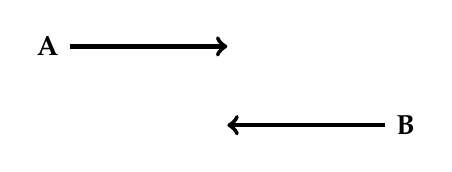
\begin{tikzpicture}[scale=2]
      \draw[ultra thick,->] (1,.5)--(2,.5) node[pos=0,left] {\textbf{A}};
      \draw[ultra thick,->] (3,0)--(2,0) node[pos=0,right]{\textbf{B}};
    \end{tikzpicture}
  \end{center}
  If Person A and Person B are moving at constant velocity relative to one 
  another (doesn't matter if they're moving towards, or away from each other)
  \begin{itemize}
  \item They cannot agree whether any events happens at the same time or not
  \item Each sees the other's clock running slow
  \item Each sees the other ``contracted'' in length along the direction of
    motion
  \end{itemize}
\end{frame}

\begin{frame}
  \frametitle{Example Problem}
  \textbf{Example 2:} A spacecraft passes Earth at a speed of \SI{2.00e8}{m/s}.
  If observers on Earth measure the length of the spacecraft to be
  \SI{554}{m}, how long would it be according to its passengers?
\end{frame}


\begin{frame}
  \frametitle{Lorentz Transformation}
  The equations for time dilation and length contraction only tell part of the
  story. In order to account for the loss of simultaneity from one reference
  frame to another, we need to use the \textbf{Lorentz transformation:}

  \vspace{-.45in}{\Large
    \begin{align*}
      x' &= \gamma(x-vt)\\
      y' &= y\\
      z' &= z\\
      t' &=\gamma\left(t-\frac{vx}{c^2}\right)
    \end{align*}
  }
  
  \vspace{-.1in}The Lorentz transformation ``solves'' many paradoxes
  (e.g.\ the twin paradox) from the time-dilation and
  length-contraction equations, but aren't really there.
\end{frame}

\begin{frame}
  \frametitle{Lorentz Transformation}
  For slow speeds $v\ll c$, Lorentz transformation reduces to the Galilean
  transformation from classical mechanics.

  \vspace{-.45in}{\Large
    \begin{align*}
      x' &= x-vt\\
      y' &= y\\
      z' &= z\\
      t' &= t'
    \end{align*}
  }
\end{frame}



\section{Rel.\ Velocity}

\begin{frame}
  \frametitle{Relative Velocity}
  \begin{itemize}
  \item Unlike in classical mechanics, velocities (speeds) do not simply add
  \item If the observer in frame $S$ measures an object moving along the
    $x$-axis at velocity $u$, then the observer in the referenfe frame $S′$
    that is moving at velocity $v$ in the $x$-direction with respect to $S$,
    will measure the object moving with velocity $u′$:

    \eq{-.2in}{
      u'=
      \frac{dx'}{dt'}=
      \frac{\gamma(dx-vdt)}{\gamma(dt-vdx/c^2)}=
      \frac{(dx/dt)-v}{1-(v/c^2)(dx/dt)}=
      \frac{u-v}{1-uv/c^2}
    }
    
  \item The other frame S will measure:
    \eq{-.2in}{
      u=
      \frac{dx}{dt}=
      \frac{\gamma(dx'+vdt')}{\gamma(dt'+vdx'/c^2)}=
      \frac{(dx'/dt')+v}{1+(v/c^2)(dx'/dt')}=
      \frac{u'+v}{1+u'v/c^2}
    }
  \end{itemize}
\end{frame}



\begin{frame}
  \frametitle{Relativistic Momentum}

  \textbf{The definition of momentum has not changed}, but in relativistic
  momentum, we must now include the effects of time dilation and/or length
  contraction:

  \eq{-.2in}{
    \boxed{\mb{p}=\frac{m\mb{v}}{\bigsqrt}=\gamma m\mb{v}}
  }
\end{frame}


\begin{frame}
  \frametitle{Relativistic Mass}
  Relativistic momentum equation show that there is a relativistic aspect to
  mass. The apparent mass $m'$ as measured by a moving observer is related to
  its rest mass (intrinsic mass, invariant mass) $m$ by the Lorentz factor:

  \eq{-.18in}{
    \boxed{m'=\frac{m}{\bigsqrt}=\gamma m}
  }
  
  The intrinsic mass has not increased, but a moving observer will see the
  object behave as if it is more massive. As $v\rightarrow c$,
  $m\rightarrow\infty$.
\end{frame}



\section[Energy]{Relativistic Energy}

%\begin{frame}
%  \frametitle{Work and Energy}
%  Einstein published a fourth paper in \emph{Annalen der Physik} on November
%  21, 1905 (received Sept.\ 27) titled ``Does the Inertia of a Body Depend Upon
%  Its Energy Content?'' (In German: Ist die Tr\"{a}gheit eines K\"{o}rpers von
%  seinem Energieinhalt abh\"{a}ngig?)
%  \begin{itemize}
%  \item Einstein deduced the most famous of equations: $E=mc^2$
%  \end{itemize}
%\end{frame}


\begin{frame}
  \frametitle{Work and Energy}
  Recall the definition of work. \textbf{This definition has not changed.}

  \eq{-.2in}{
    W=\int\mb{F}\cdot d\mb{x}=\int\frac{d\mb{p}}{dt}\cdot \mb{dx}
  }

  \vspace{-.1in}Since we now have a relativistic expression for momentum, we
  substitute that new expression into the expression for force, and then
  integrate.

  \vspace{.2in}Doing the integral gives a surprisingly simple expression for
  kinetic energy $K$:
  
  \eq{-.15in}{
    W=\gamma mc^2-mc^2
  }

\end{frame}


\begin{frame}
  \frametitle{Work and Energy}

  We know from the work-kinetic energy theorem that the work $W$ done is equal
  to the change in kinetic energy $K$, therefore
 
  \eq{-.2in}{ \boxed{K=m'c^2-mc^2} }

  \vspace{-.1in}
  \begin{center}
    \begin{tabular}{l|c|c}
      \rowcolor{pink}
      \textbf{Variable} & \textbf{Symbol} & \textbf{SI Unit}\\ \hline
      Kinetic energy of an object & $K$  & \si{\joule}\\
      Relativistic mass (measured in moving frame) & $m'$ & \si{\kilo\gram}\\
      Rest mass (measured in stationary frame) & $m$  & \si{\kilo\gram}\\
      Speed of light              & $c_0$ & \si{\metre\per\second}
    \end{tabular}
  \end{center}

  \textbf{The full integration is shown in the long version of the slides. The
    integral is not very complicated, but it does require some experience with
    intgral calculus.}
\end{frame}

\begin{frame}
  \frametitle{Relativistic Energy}
  \framesubtitle{What This All Means}
  {\Large
    \begin{displaymath}
      \boxed{K=m'c^2-mc^2}
    \end{displaymath}
  }

  \begin{itemize}
  \item\vspace{-.3in}\textbf{rest energy}:
  
    \eq{-.4in}{ E_0=mc^2 }
  \item\textbf{total energy}:
    
    \eq{-.3in}{
      E_T=m'c^2=\gamma mc^2
    }
  \item Kinetic energy is the difference between total energy and rest energy:

    \eq{-.3in}{
      K=E_T-E_0
    }
  \end{itemize}
\end{frame}


\begin{frame}
  \frametitle{Relativistic Energy}
  \framesubtitle{What This All Means}
  
  \eq{-.2in}{
    \boxed{E=mc^2}
  }

  \textbf{Mass-energy equivalence}:
  \begin{itemize}
  \item Whenever there is a change of energy, there is also a change of mass
  \item ``Conservation of mass'' and ``conservation of energy'' must be
    combined into a single concept of \textbf{conservation of mass-energy}
  \item Mass-energy equivalence doesn't merely mean that mass can be converted
    into energy, and vice versa (although this is true), but rather, one can be
    converted into the other
    \textbf{because they are fundamentally the same thing}
  \end{itemize}
\end{frame}



\begin{frame}
  \frametitle{Example Problem}
  \textbf{Example 3:} An electron has a rest mass of \SI{9.11e-31}{\kilo\gram}.
  In a detector, it behaves as if it has a mass of \SI{12.55e-31}{\kilo\gram}.
  How fast is that electron moving relative to the detector?
\end{frame}


\begin{frame}
  \frametitle{Energy-Momentum Relation}
  The \textbf{energy-momentum relation} relates an object's rest (intrinsic)
  mass $m$, total energy $E$, and momentum $p$:

  \eq{-.2in}{
    \boxed{E^2=p^2c^2+m^2c^4}
  }
  \begin{center}
    \begin{tabular}{l|c|l}
      \rowcolor{pink}
      \textbf{Quantity} & \textbf{Symbol} & \textbf{SI Unit} \\ \hline
      Total energy   & $E$ & \si{\joule} (joules) \\
      Momentum       & $p$ & \si{\kilo\gram\metre/\second}
      (kilogram meters per second) \\
      Rest mass      & $m$ & \si{\kilo\gram} (kilogram)\\
      Speed of light & $c$ & \si{\metre/\second} (meter per second)
    \end{tabular}
  \end{center}

  \textbf{The derivation of this expression is shown in the long version of the
  slides.}
\end{frame}

%\begin{frame}
%  \frametitle{Energy-Momentum Relation}
%  This equation is derived using the expression for relativistic momentum:
%
%  \eq{-.2in}{
%    p=\gamma mv=\frac{mv}{\bigsqrt}
%  }
%  If we square both sides of the equation, we get:
%
%  \eq{-.2in}{
%    p^2=\gamma^2m^2v^2=\frac{m^2v^2}{1-\left(\frac {v}{c}\right)^2}
%  }
%\end{frame}
%
%\begin{frame}
%  \frametitle{Energy-Momentum Relation}
%  Solving for $v^2$ and substituting it back into the Lorentz factor, we
%  obtain its alternative form in terms of momentum and mass:
%
%  \eq{-.2in}{
%    \gamma =\sqrt{1+\left(\frac {p}{mc}\right)^2}
%  }
%  Inserting this form of the Lorentz factor into the energy equation, we have
%
%  \eq{-.2in}{
%    E=mc^2 \sqrt{1+\left(\frac{p}{mc}\right)^2}
%  }
%
%  Which is the same equation as in the last slide.
%\end{frame}
%
%\begin{frame}
%  \frametitle{Energy-Momentum Relation}
%
%  In the \textbf{stationary frame of reference}, (rest frame,
%  center-of-momentum frame) the momentum is zero, so the equation simplifies to
%
%  \eq{-.2in}{
%    E=mc^2
%  }
%  where $m$ is the rest mass of the object.
%
%  \vspace{.2in}If the object is \textbf{massless}, as is the case for a
%  \textbf{photon}, then the equation reduces to
%
%  \eq{-.4in}{
%    E=pc
%  }
%\end{frame}



\begin{frame}
  \frametitle{Kinetic Energy--Classical vs.\ Relativistic}
  \begin{columns}
    \column{.5\textwidth}
    \textbf{Relativistic:}
    {\Large
      \begin{displaymath}
        K=\frac{mc^2}{\bigsqrt}-mc^2
      \end{displaymath}
    }
    
    \column{.5\textwidth}
    \textbf{Newtonian:}
    {\Large
      \begin{displaymath}
        K=\frac{1}{2}mv^2
      \end{displaymath}
    }
  \end{columns}
  If space and time are indeed relative quantities, then the relativistic
  equation for $K$ must apply to all velocities
\end{frame}


\begin{frame}
  \frametitle{Kinetic Energy---Classical vs.\ Relativistic}
  Applying the \textbf{binomial series expansion} to $\gamma$ gives a
  series representation of kinetic energy $K$:

  \vspace{-.3in}{\Large
    \begin{align*}
      K &= mc^2
      \left(1+\frac{1}{2}\frac{v^2}{c^2}+\frac{3}{8}\frac{v^4}{c^4}+\cdots
      \right) - mc^2\\
      &\approx\frac{1}{2}mv^2+\frac{3mv^4}{8c^2}+\cdots
    \end{align*}
  }
  
  For $v\ll c$, we can ignore the high-order terms. The leading term reduces to
  the Newtonian expression.
\end{frame}


\begin{frame}
  \frametitle{Comparing Classical and Relativistic Energy}
  \begin{columns}
    \column{.5\textwidth}
    In classical mechanics:
    {\Large
      \begin{displaymath}
        K=\frac{1}{2} mv^2
      \end{displaymath}
    }
    In relativistic mechanics:
    {\Large
      \begin{displaymath}
        K=\gamma mc^2-mc^2
      \end{displaymath}
    }
    
    \column{0.5\textwidth}
    \pic{.85}{graphics/e_k.png}
  \end{columns}

  The classical expression is accurate for speeds up to $v\approx 0.3c$.
\end{frame}

\begin{frame}
  \frametitle{Example Problem}
  \textbf{Example 4:} A rocket car with a mass of \SI{2.00e3}{kg} is accelerated
  from rest to \SI{1.00e8}{m/s}. Calculate its kinetic energy:
  \begin{enumerate}
  \item Using the classical equation
  \item Using the relativistic equation
  \end{enumerate}
\end{frame}

\end{document}
